\maketitle
\setcounter{page}{1}
\tableofcontents
\newpage
\pagenumbering{arabic}
\section{Theorie}
\section{Auswertung}
\subsection{Eichung des B-Feldes}
Die Messwerte sowie eine graphische Darstellung mit Fit sind in Abbildung \ref{A_Abb:1}
dargestellt. Der Fit wurde nach least-squares durch die Funktion $\textsc{polyfit}$
aus dem $\textsc{Python}$\footnote{Version: 3.6.3} Paket
$\textsc{numpy}$\footnote{Version: 1.13.3} mit einem Polynom 3. Grades erstellt.

\begin{figure}[h!]
  \centering
  \subcaptionbox{Messwerte. \label{}}[0.20\textwidth]{
  \centering
  \begin{tabular}{c c}
    \toprule
    $I / \si{\ampere}$ & $B / \si{\milli\tesla}$ \\
    \midrule
    0 & 5.05 \\
    1 & 64 \\
    2 & 139 \\
    3 & 191 \\
    4 & 237 \\
    5 & 308 \\
    6 & 363 \\
    7 & 423 \\
    8 & 486 \\
    9 & 533 \\
    10 & 599 \\
    11 & 662 \\
    12 & 720 \\
    13 & 770 \\
    14 & 821 \\
    15 & 870 \\
    16 & 915 \\
    17 & 949 \\
    18 & 985 \\
    19 & 1006 \\
    20 & 1032 \\
    \bottomrule
  \end{tabular}
  }
  \subcaptionbox{Grafische Darstellung mit Regression. \label{}}[0.78\textwidth]{
  \centering
  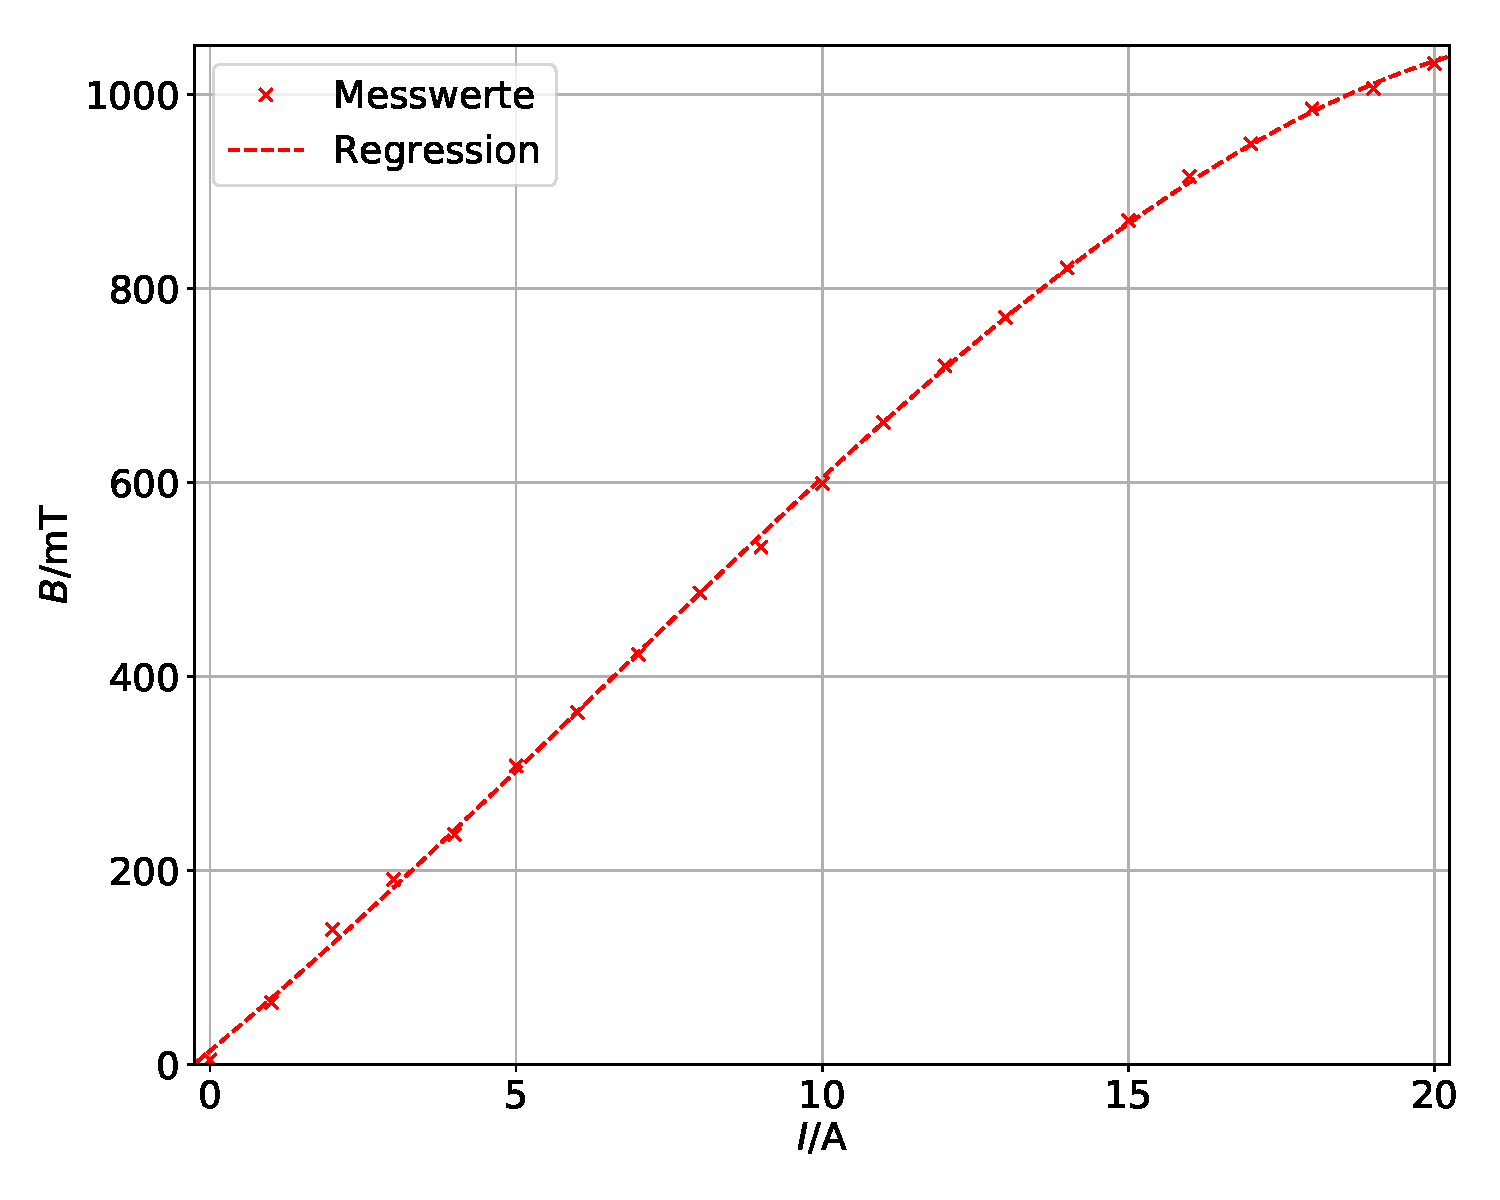
\includegraphics[width=0.78\textwidth]{B_Feld.pdf}
  }
  \caption{Magnetfeldeichung.}
  \label{A_Abb:1}
\end{figure}

Die Fitparameter mit Fehlern lauten:
\begin{align}
\begin{split}
  a_3 &= \SI{-0.072(9)}{\milli\tesla\per\cubic\ampere}\\
  a_2 &= \SI{1.350(269)}{\milli\tesla\per\square\ampere}\\
  a_1 &= \SI{52.750(2282)}{\milli\tesla\per\ampere}\\
  a_0 &= \SI{14.035(5142)}{\milli\tesla}.
  \label{A_eq:1}
\end{split}
\end{align}
Mit den Werten in \eqref{A_eq:1} folgt also als genäherte Feldstromstärke - Magnetfeld
- Beziehung:
\begin{equation}
  B(I) = a_3 \cdot I^3 + a_2 \cdot I^2 + a_1 \cdot I + a_0
\end{equation}



\newpage
\nocite{*}
\printbibliography
